\section{Power over Ethernet}
Bei Power over Ethernet wird die Energieversorgung über eine herkömmliche Cat5-Ethernetleitung mitgeführt.
Dadurch wird eine weitere Versorgungsleitung eingespart.
Eine Ethernet Leitung besteht aus acht Adern, wobei je zwei Adern zu einem Adernpaar verdrillt sind.
Je nach Geschwindigkeit der Datenübertragung werden nur vier oder alle acht Adern für die Datenübertragung verwendet.
Das bedeutet, bei geringeren Übertragungsraten können die freien Adern zur Versorgung genutzt werden.
Wenn alle acht zur Datenübermittlung verwendet werden, müssen vier Adern für Datenübertragung \emph{und} Energieversorgung genutzt werden.\par

Grundsätzlich wird zwischen vier verschiedenen Typen unterschieden:
\paragraph{Type 1, \ac{poe}:}
Der Standard IEEE 802.3af gilt nur für 10 Mbit/s und 100 Mbit/s.
Das bedeutet, dass nur die Adernpaare 1/2 und 3/6 für die Datenübertragung genutzt werden und die beiden anderen Adernpaare unbenutzt sind.
Je Adernpaar ist ein Strom von maximal 175 mA vorgesehen. Bei zwei Adernpaaren ist das in Summe ein Strom von 350 mA.
Beim Einschalten sind kurzzeitig 400 mA erlaubt.
Die maximale Leistungsaufnahme beträgt 15,4 Watt pro Switch-Port.

\paragraph{Type 2, \ac{poep}:}
Mit IEEE 802.3at eignet sich Power-over-Ethernet auch für 1000 Mbit/s (Gigabit).
Gleichzeitig wird die Leistung fast verdoppelt.
IEEE 802.3at verspricht eine Leistung bis 25,5 Watt pro Port.
Dabei wird die Minimalspannung von 44 auf 50 Volt erhöht.
Der maximale Strom wurde von 350 mA auf 600 mA erhöht.
Bei diesen hohen Leistungen wird ein Cat5e/6-Kabel empfohlen.

\paragraph{Type 3 \& 4, \ac{poepp}:}
Den Standard IEEE 802.3bt bezeichnet man als Four-Pair-Power-over-Ethernet. Die Kurzschreibweise \ac{poepp} oder \aca{poepp}.
Bisher nutzt Power-over-Ethernet nur zwei der vier Aderpaare eines Twisted-Pair-Kabels. Mit \ac{poepp} werden alle Adern der vorhandenen Kabel zur Leistungsübertragung verwendet. Damit steigt die Leistung auf 70 bis 100 Watt.

Aus den verschiedenen Typen ergeben sich zwei Arten der Energiespeisung:
\paragraph{Spare-Pairs-Verfahren:}
Das Spare-Pairs-Verfahren verwendet die beiden unbenutzten Adernpaare im Kabel (4/5 und 7/8) für die Stromversorgung. Die Übertragung von Strom und Daten sind voneinander getrennt. Diese Art kann nur bei Type 1 und Type 2 verwendet werden.

\paragraph{Phantom-Speisung:}
Bei der Phantom-Speisung werden die datenführenden Adern im Kabel verwendet. Phantom-Speisung bedeutet, dass der Strom für die Energieversorgung dem Datensignal überlagert wird. Das Power-Device muss die Entkopplung übernehmen, was fehleranfällig, aufwendig und teuer ist.
Wenn alle Adernpaare des Kabels für die Datenübertragung verwendet werden, d.h. es wird Type 3 oder Type 4 angewendet, dann ist man zwangsläufig auf die Phantom-Speisung angewiesen. Hierbei ist der Strom pro Adernpaar und somit die Gesamtleistung begrenzt.

\begin{table}[htbp!]
	\centering
	\begin{tabular}{lccc}
		\toprule
		Type & \acs{poe} & \acs{poep} & \acs{poepp} \\
		\midrule
		Ausgangsspannung & 36-57 V & 42.5-57 V & 42.5-57 V \\
		\midrule
		Ausgangsstrom Betrieb & 350 mA & 600 mA & 2x 960 mA \\
		\midrule
		Ausgangsstrom Startmodus & 400 mA & 400 mA & ?\textsuperscript{*} \\
		\midrule
		Leistung der (\acs{pse})-Versorgung & max. 15.4 W & max. 30 W & 45/60/75/90 W \\
		\midrule
		Leistung am Endgerät (\acs{pd}) & max. 12.95 W & max. 25.5 W & 40/51/62/71 W\\
		\midrule
		\acs{pse}-Klasse & 1, 2, 3 & 4 & 5, 6, 7, 8 \\
		\midrule
		unterstützte Endgeräte (\acs{pd}-Type) & 1 & 1 und 2 & 1, 2, 3, 4 \\
		\midrule
		Benutzte Adernpaare & 2 & 2 & 2 und 4 \\
		\bottomrule
	\end{tabular}\bigskip\par
	\textsuperscript{*}in Fachartikel \citetitle{elektropraktiker-poe} nicht behandelt
	\caption{Vergleich PoE-Typen \cite[vgl.][]{elektropraktiker-poe}}
	\label{tab:poe-types}
\end{table}

\section{Spannungsregler}
Ein Spannungsregler stabilisiert eine elektrische Spannung.
Er wird eingesetzt, wenn eine konstante Betriebsspannung benötigt wird.
Grundsätzlich arbeitet ein Spannungsregler mit einem Leistungstransistor, der so angesteuert wird, dass die gewünschte Ausgangsspannung zu Stande kommt.\par

Es gibt zwei Arten von Spannungsregler:
\paragraph{Linearregler:}
Beim Linearregler wird der Leistungstransistor als veränderbarer Widerstand genutzt.
Über einen Regelkreis wird eine Veränderung der Ausgangsspannung, z.B. Laständerung, festgestellt.
Daraufhin ändert der Transistor seinen Innenwiderstand, um die Veränderung auszugleichen.\par

\paragraph{Schaltregler:}
Der Schaltregler hingegen nutzt den Leistungstransistor als Schalter.
Er schaltet mit einer Frequenz von mehreren kHz bis MHz und erzeugt somit ein \ac{pwm} Signal.
Dieses Signal wird anschließend mit einer Induktivität geglättet, um einen konstanten Strom zu erzielen.
Mit der Pulsbreite wird der Effektivwert des PWM-Signals und damit die Höhe der geglätteten Spannung variiert.\par

\section{Surface Mounting Technology}
Bei der klassischen \ac{tht}-Technologie werden die Bauteilanschlüsse durch Löcher in der Platine gesteckt und mit kreisförmigen Lötpads auf der gegenüberliegenden Seite verlötet.
Im Gegensatz dazu sind bei \ac{smd}-Platinen Bauteile und Lötpads auf derselben Platinenseite, weshalb keine Bohrungen mehr erforderlich sind.
Die Bauteilanschlüsse werden flach mit dem rechteckigen Lötpad verbunden.
Die Verlötung findet mithilfe von Heißluft statt.
Die fertig bestückten Platinen werden in einen Reflow-Ofen gelegt und auf die Schmelztemperatur der Lötpaste erhitzt.

\subsection{Entwicklung}
In den 1960ern wurde die Oberflächenmontagetechnik (\ac{smt}) von IBM entwickelt und fand ihre ersten Anwendungen in den Saturn- und Apollo-Missionen.
In den 1970ern wurde die \ac{smt} erstmals genormt, wodurch sich die Technologie im kommerziellen Sektor verbreiten konnte.
Die \ac{smt} bietet gegenüber der herkömmlichen \ac{tht} einige Vorteile:
\paragraph{Vorteile:}
\begin{itemize}
	\item Miniaturisierung, aufgrund der geringeren Größe der Bauteile können Platinen und somit auch Endgeräte kleiner und kompakter gebaut werden.
	\item Auch das Gewicht wird durch die Verkleinerung der Bauelemente stark reduziert.
	\item Der Bauteilabstand kann verkleinert werden, dadurch verbessert sich der Platzverbrauch weiter.
	\item Die Hochfrequenzeigenschaft wird durch die kürzeren Übertragungswege zwischen den Bauteilen verbessert.
	\item Die Fertigung der Platinen kann mit \ac{smd} besser automatisiert werden, da die Positionierung der Bauelemente nicht so genau sein muss, wie bei \ac{tht}.
	Die Bauteile werden beim Verlöten durch die Oberflächenspannung des Lötzinns in die korrekte Position gezogen.
	\item Einfache doppelseitige Bestückung von Platinen, da kein Platz von Anschlüssen von Bauteilen auf der anderen Platinenseite verbraucht wird.
\end{itemize}

\paragraph{Nachteile:}
\begin{itemize}
	\item Anschlüsse an der Unterseite von Bauteilen können nur durch Röntgen überprüft werden.
	\item Das Heißluftlötverfahren erhitzt nicht nur die Lötstelle, sondern das gesamte Bauteil.
 	Dadurch besteht ein höheres Risiko, dass dieses beim Anlöten zerstört wird.
 	\item Große Bauelemente benötigen zusätzliche Fixierung, da die Lötstelle der mechanischen Belastung nicht standhält.
	Aufgrund der vielen Vorteile gegenüber \ac{tht} fand die \ac{smt} in der Digital- und Computertechnik anfänglich häufige Anwendung.
	Anfang der 1980er begannen die ersten Unternehmen mit der automatischen Fertigung von \ac{smd}-Platinen, wodurch die Herstellungskosten weiter gesenkt wurden.	
\end{itemize}

\subsection{Bauteilcodes}
Grundsätzlich werden alle elektronischen Bauteile in die beiden Untergruppen aktive und passive Bauelemente unterteilt.\par

Aktive Bauelemente können Signale verstärken oder erzeugen. Die benötigte Energie kommt aus einer zusätzlichen Versorgung durch elektrische oder einer anderen Energieform. Beispiele für aktive Bauteile sind Transistoren, \acp{ic}, Photovoltaikzellen, \dots\par

Passive Bauelemente können im Gegensatz zu aktiven Bauteilen selbst keine Signale erzeugen oder verstärken. Sie benötigen keine zusätzliche Energieversorgung, um zu funktionieren. Beispiele für diese Art sind Widerstände, Kondensatoren und Spulen.

\subsubsection{Passive Bauteile}
Für passive Bauelemente gibt es vier wichtige Bezeichnungen:
\paragraph{Chip:}
Dies ist die Standard Bauform für unter anderem Keramik- und Tantal-Konden\-satoren, Induktivitäten sowie nichtlineare und lineare Widerstände.
Ein Chip ist ein quaderförmiges Bauteil, das auf der Platine aufliegt. In die Bezeichnung fließt nur die bauliche Größe ein.
Die Größe wird mit einem metrischen Code angegeben, z.B. „0603“, die Ziffer „06“ steht für die Länge und „03“ für die Breite.
In diesem Beispiel bedeutet das, dass das Bauteil 0,6 mm lang und 0,3 mm breit ist.
\begin{figure}[htbp!]
	\centering
	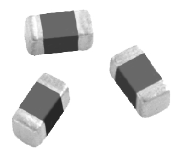
\includegraphics{images/technische_grundlagen/chip.png}
	\caption{Chip-Bauform \cite[vgl.][]{vishay-chip}}
\end{figure}

\paragraph{\ac{melf}:}
Die \ac{melf} Bauform ist im Gegensatz zur Chip-Bauform zylinderförmig, liegt aber ebenfalls flach auf der Platine auf.
Diese Bauform ist deutlich größer als die Chip Variante, dafür bietet sie elektrische Vorteile.
Die \ac{melf} Bauteile haben eine bessere Spannungsfestigkeit, höhere Impulsstrombelastbarkeit und eine bessere Temperaturstabilität.
Im Fehlerfall sind in dieser Bauweise die Widerstände so ausgelegt, dass sie in jedem Fall hochohmig werden und dadurch Schäden an anderen Bauteilen verhindern können.
Beim Lötvorgang hingegen kann es bei \ac{melf} Bauteilen dazu kommen, dass sie wegrollen. Daher werden sie meist vor dem Lötvorgang festgeklebt.
\begin{figure}[htbp!]
	\centering
	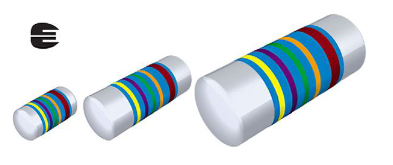
\includegraphics{images/technische_grundlagen/melf.png}
	\caption{\ac{melf}-Bauform \cite[vgl.][]{vishay-melf}}
\end{figure}

\paragraph{\ac{sod}:}
Wie der Name schon sagt ist das eine Gehäuseform, welche ausschließlich für Dioden verwendet wird. Die Bauteile sind entweder wie bei \ac{melf} zylindrisch (z.B. \ac{sod}-80 oder Mini\ac{melf}) oder quaderförmig mit Anschlussfahnen (z.B. \ac{sod}-123) ausgeführt.
\begin{figure}[htbp!]
	\centering
	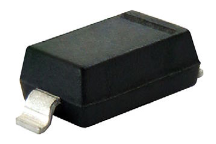
\includegraphics{images/technische_grundlagen/sod-123.png}
	\caption{\ac{sod}-123-Bauform \cite[vgl.][]{vishay-sod-123}}
\end{figure}

\paragraph{\ac{vchip}:}
Ein \ac{vchip} ist ebenfalls zylindrisch, jedoch werden diese Bauteile stehend montiert.
Diese Bauform wird häufig bei Aluminium-Elektrolytkondensato\-ren verwendet und können dabei große Abmessungen erreichen.
\begin{figure}[htbp!]
	\centering
	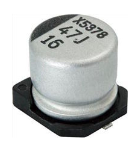
\includegraphics{images/technische_grundlagen/vchip.png}
	\caption{\ac{vchip}-Bauform \cite[vgl.][]{vishay-vchip}}
\end{figure}

\subsubsection{Aktive Bauteile}
Für aktive Bauelemente (\acp{ic}) gibt es wesentlich mehr Bauformen und Bezeichnungen. Daher werden hier nur einige wichtige aufgeführt.
\paragraph{\ac{sot}:}
Diese Bauform wird ausschließlich für Transistoren verwendet. Sie hat drei oder vier Anschlüsse, wobei der vierte nur zum Abführen entstandener Wärme dient. Das Bauteil ist in dieser Bauform in einem quaderförmigen Kunststoff-Gehäuse verschweißt.
\begin{figure}[htbp!]
	\centering
	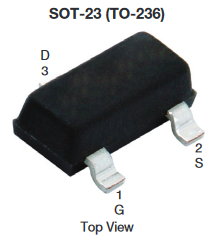
\includegraphics{images/technische_grundlagen/sot-23.png}
	\caption{\ac{sot}-23-Bauform \cite[vgl.][]{vishay-sot}}
\end{figure}

\paragraph{\ac{soic}:}
Bauteile in dieser Ausführung ähneln einem herkömmlichen \ac{dip}-Gehäuse, da der Anschlussabstand bei beiden Formen gleich groß ist. Dieser Gehäusetyp wird vor allem für \acp{ic} verwendet.
\begin{figure}[htbp!]
	\centering
	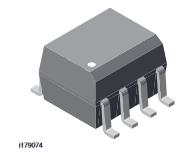
\includegraphics{images/technische_grundlagen/soic.png}
	\caption{\ac{soic}-Bauform \cite[vgl.][]{vishay-soic}}
\end{figure}

\paragraph{\ac{sop}:}
Dies ist eine kleinere Form der \ac{soic}-Bauform und wird ebenso hauptsächlich für \acp{ic} verwendet. Diese Ausführung bekommt je nach Baugröße einen oder mehrere zusätzliche Buchstaben vorangestellt.
\begin{figure}[htbp!]
	\centering
	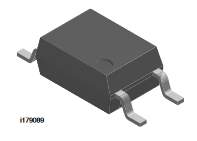
\includegraphics{images/technische_grundlagen/sop.png}
	\caption{\ac{sop}-Bauform \cite[vgl.][]{vishay-sop}}
\end{figure}

%Entwicklung (zuerst tht, 1960 abgelöst durch smd, erfinder->IBM, Saturn- u. Apollo-Mission)
%Verwendung in Bereich Digitaltechnik, Raumfahrt; Bereiche für tht?
\subsection{Mögliche Fertigungsfehler}
\subsubsection{Grabstein-Effekt:} %Bauteil hebt sich beim anlöten von der Platine
Bei dem sogenannten Grabsteineffekt handelt es sich um einen Fehler, der bei der Verlötung der Bauteile mit der Platine auftreten kann.
Ein Bauteil mit zwei Anschlüssen wird auf einer Seite angelötet.
Aufgrund der Oberflächenspannung des Lötzinns hebt sich das Bauelement auf einer Seite der Platine ab.
Diese Position lässt das Bauteil wie einen kleinen Grabstein erscheinen.\par

Um diesen Effekt entgegenwirken zu können, wird darauf geachtet, dass beide Lötstellen zeitgleich erhitzt werden.
\begin{figure}[htbp!]
	\centering
	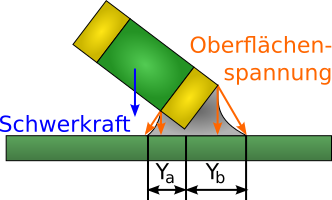
\includegraphics[width=.5\linewidth]{images/technische_grundlagen/grabsteinEffekt.png}%https://upload.wikimedia.org/wikipedia/commons/9/97/Tombstone_Effect_DE.svg
	\caption{Grabstein-Effekt \cite{wikimedia-grabstein}}
\end{figure}

\subsubsection{Popcorn-Effekt:} %aufgenommene Luftfeuchtigkeit expandiert beim Heißluftlöten und zerstört das bauteil
Ein feuchteempfindliches Bauteil, wie zum Beispiel eine Rohplatine oder das Trägermaterial eines Prozessors, welches außerhalb der vor Feuchte schützenden Verpackung gelagert wird, neigt zum Popcorn Effekt.
Das Bauteil nimmt die Feuchtigkeit aus der Umgebung auf und speichert diese.
Beim Löten verdampft das Wasser und bläht das Bauteil aufgrund der Ausdehnung auf.
Das Ausdehnen führt u. a. zu Rissen im Gehäuse oder Delaminierung der Kupferschicht.\par

Diese Fehler führen meist zur Zerstörung des Bauteils und können erst nach der Fertigung diagnostiziert werden.
Vorbeugend ist auf eine korrekte Lagerung der Komponenten zu achten.
\begin{figure}[htbp!]
	\centering
	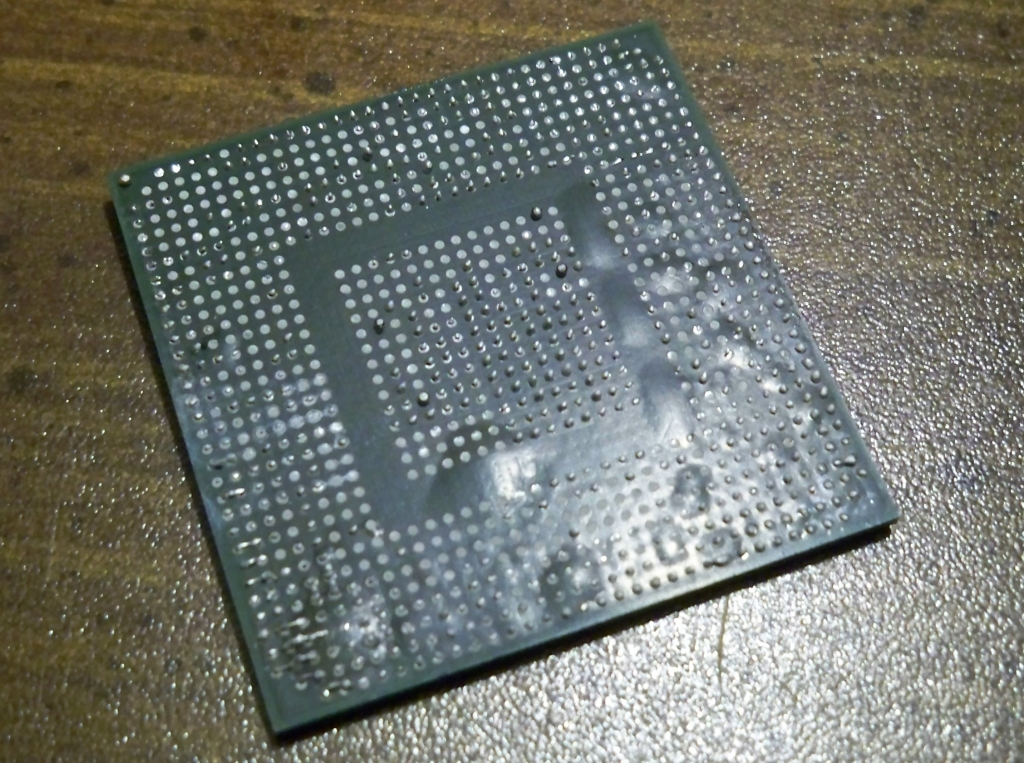
\includegraphics[width=.5\linewidth]{images/technische_grundlagen/popcornEffekt.jpg}%https://upload.wikimedia.org/wikipedia/commons/9/97/PopcornBGA.jpg
	\caption{Popcorn-Effekt \cite{wikimedia-popcorn}}
\end{figure}

\section{Serielle Schnittstellen}
\subsection{Universal Asynchronous Receiver/Transmitter}
\ac{uart} ist ein universell einsetzbarer elektronischer Baustein, der Systemeinheiten mit parallelem Übertragungsmodus an serielle Übertragungswege anpasst.
Mit dem \ac{uart} werden in Personal Computern (PC) die parallel anfallenden Daten in serielle Datenströme umgewandelt, die dann an den seriellen Schnittstellen (\acs{com}, \acs{lpt}, \acs{ide-drive}, usw.) für die angeschlossenen Peripheriegeräte und für die Datenübertragung über Modems zur Verfügung stehen. \cite{itwissen-uart}\par

Der \ac{uart}-Datensatz besteht aus 11 Bit, einem Startbit, acht Datenbits, einem Paritätsbit und einem Stoppbit.
Der \ac{uart} selbst besteht aus zwei \ac{fifo}-Puffern, die sende- und empfangsseitig die ein- und ausgehenden Datensignale zwischenspeichern.
Je nach Breite des Datenbusses gibt es Wandler für 8-Bit und 16-Bit mit Übertragungsraten von 19,2 kbit/s, 56 kbit/s (\ac{uart}16450) und 128 kbit/s (\ac{uart}16650D). \cite{itwissen-uart}\par
\begin{figure}[htbp!]
	\centering
	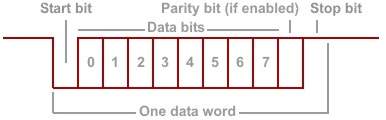
\includegraphics[width=.9\linewidth]{images/technische_grundlagen/tide_uart_data.png}
	\caption{Aufbau eines \ac{uart}-Frames \cite{tibbo-uart}}
\end{figure}

\ac{uart} wurde für diese Anwendung ausgewählt, wegen der Einfachheit der Verdrahtung.
Die Kommunikation der Geräte findet über nur zwei Datenleitungen statt, dadurch werden Verbindungen zwischen der Platine und dem \ac{rpi} eingespart.
\ac{uart} wird vom \ac{rpi} und Mikrocontroller unterstützt.


\subsection{Serial Peripheral Interface}
Das Serial Peripheral Interface, kurz \ac{spi} oder auch Micro Wire genannt, ist ein Bussystem bestehend aus drei Leitungen für eine serielle synchrone Datenübertragung zwischen verschiedenen \acp{ic}. \cite{mikrocontroller-spi}\par

SPI-Bausteine kommunizieren im Vollduplex-Modus.
Das System verwendet eine Master-Slave-Architektur mit einem einzigen Master.
Der Bus besteht aus folgenden Leitungen
\begin{itemize}
	\item \ac{mosi}
	\item \ac{miso}
	\item \ac{sck} - Schiebetakt	
\end{itemize}

Zusätzlich zu diesen drei Leitungen wird für jeden Slave eine \ac{ss} genannte Leitung benötigt, durch die der Master den Slave zur aktuellen Kommunikation selektiert.
Dies geschieht dadurch, dass der Master die \ac{ss}-Leitung von High nach Low zieht.
Oft ist mit dieser Aktivierung durch den Master auch eine Benachrichtigung für den Slave verbunden, mit der ihm mitgeteilt wird, dass jetzt eine Nachricht beginnt, das nächste Byte also zum Beispiel als Kommando aufzufassen ist. \cite{mikrocontroller-spi}\par

Die Übertragung geschieht so, dass der Master seine Datenleitung (\ac{mosi}) auf den Pegel des nächsten Bits bringt und dann an der \ac{sck} Leitung einen Puls ausgibt.
Gleichzeitig wird vom Master der Pegel an der Datenleitung vom Slave zum Master überwacht und ihr Zustand als nächstes einzulesendes Bit aufgefasst.
Üblicherweise gibt es zumindest beim Master mehrere Einstellungen, die festlegen, welches der Grundzustand dieser \ac{sck} Leitung sein soll und welche Flanke des Taktes zur Datenübernahme herzunehmen ist (die steigende oder die fallende).
Bei einigen Slaves ist diese Einstellung ebenfalls möglich, oft ist es aber so, dass per \ac{spi} anzusprechende \ac{ic} eine feste Einstellung benutzen, an die sich der Master anpassen muss. \cite{mikrocontroller-spi}\par

Für den \ac{spi}-Bus gibt es kein festgelegtes Protokoll.
Die Taktpolarität und Phase können ebenfalls von Slave zu Slave unterschiedlich sein.
Der \ac{spi}-Bus kann mit einer Taktfrequenz von vielen Megahertz betrieben werden.
Es gibt viele verschiedene \acp{ic}, die als Slave an dem \ac{spi}-Bus betrieben werden können. Diese gehen von einfachen Schieberegistern bis hin zu \acp{rtc} oder Displaytreibern mit vorgegebenem Protokoll.
Unter anderem werden die meisten AVR-Microcontroller von Atmel über \ac{spi} programmiert. \cite{mikrocontroller-spi}\par

\section{Audio-Verstärker Class D}
Mit Class-D wird ein bestimmtes Schaltungsdesign von Audio-Verstärkern bezeichnet, die ein \ac{pwm}-Signal erzeugen und daher auch als \ac{pwm}-Verstärker bekannt sind. \cite{fairaudio-classd}\par

Bei einem herkömmlichen Transistorverstärker enthält die Ausgangsstufe Transistoren, die den momentanen kontinuierlichen Ausgangsstrom liefern.
Zu den vielen möglichen Implementierungen für Audiosysteme gehören die Klassen A, AB und B.
Im Vergleich zu Designs der Klasse D ist die Verlustleistung der Ausgangsstufe selbst in den effizientesten linearen Ausgangsstufen groß.
Dieser Unterschied verleiht der Klasse D in vielen Anwendungen erhebliche Vorteile, da die geringere Verlustleistung weniger Wärme erzeugt, Platz und Kosten auf der Leiterplatte spart und die Batterielebensdauer in tragbaren Systemen verlängert.\par

Ein symmetrisch arbeitender Dreiecksgenerator schwingt mit einer typischen Frequenz von ca. 250 kHz bis zu einigen MHz, dessen Pegel von einem Komparator mit dem Pegel des zu verstärkenden Eingangssignals verglichen wird. 
Der Komparator verwandelt das analoge Tonsignal in eine Rechteckschwingung, wie in dem Blockdiagramm zu erkennen ist.\par

Ist das Dreiecksignal größer als das Tonsignal, springt der Ausgang auf low, ist es kleiner, springt er auf high. 
Die maximale Impulsbreite ist dabei kleiner als die Zykluszeit der Arbeitsfrequenz und kann somit nie länger als ein Taktzyklus ein- oder ausgeschaltet (high oder low) sein. Das Tonsignal liegt nun im Tastverhältnis des PWM-Signals vor. 
Der Mittelwert ist dadurch exakt proportional zum Tonsignal.\par

Dieses PWM-Signal wird der Endstufe zugeführt, in welcher die eigentliche Verstärkung stattfindet, bestehend aus zwei Leistungstransistoren im Schaltbetrieb für je eine positive und eine negative Halbwelle.
Ein Class-D-Verstärker ist entweder als Halbbrücke mit zwei Transistoren aufgebaut oder mit vier Transistoren als Vollbrücke (H-Brücke) ausgeführt.

\begin{figure}[htbp!]
	\centering
	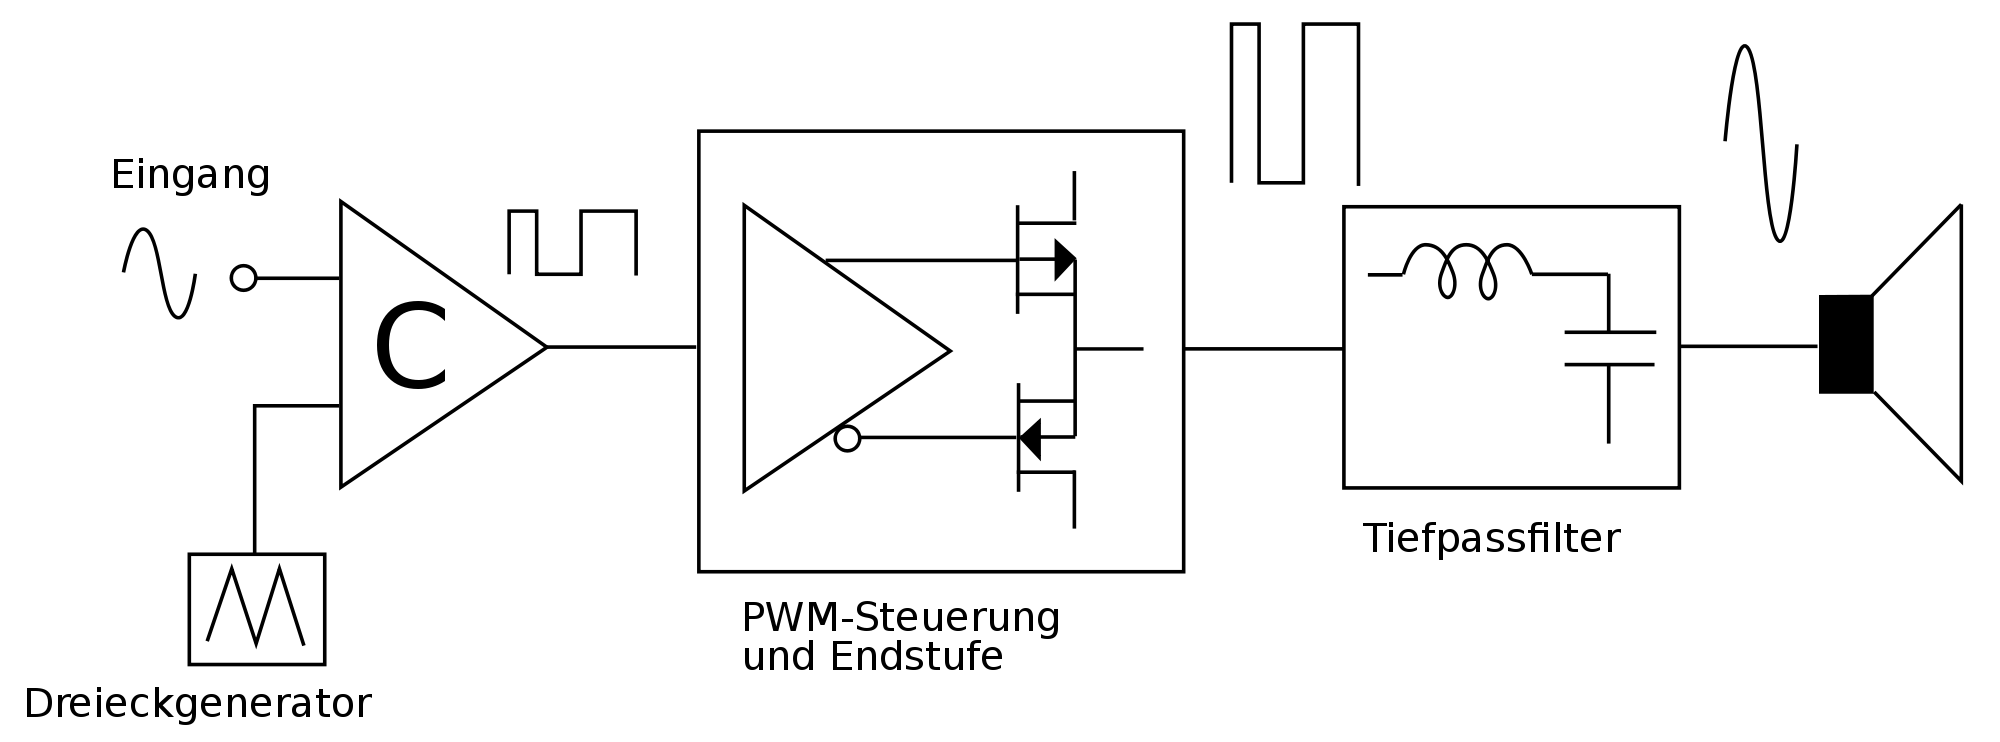
\includegraphics[width=.9\linewidth]{images/technische_grundlagen/class-d-schematisch.png}
	\caption{Schematische Darstellung Class-D \cite{wikimedia-pwm-amp}}
\end{figure}
%falls noch mehr text benötigt wird: erklärungen auf website